\chapter{Introduction\label{chap:intro}}
\localtoc

\section{Context and Motivation\label{sec:intro.context}}

Modern information security is made difficult by the scale, complexity, and heterogeneity of information systems.
Because security by design in these conditions is a considerable challenge, security agencies also recommend complementary measures.
For instance, the NIST Cybersecurity Framework~\cite{nationalinstituteofstandardsandtechnology_NISTCybersecurityFramework_2024} suggests a five-stage lifecycle for managing risks in information systems: identify, protect, detect, respond, and recover.

The \emph{detection} and \emph{response} stages can significantly benefit from the recent advances in \gls{ai} and \gls{ml}, enabling the analysis of more complex behaviors.
Yet, because organizations usually face similar threats, including large-scale campaigns such as Mirai in 2016 or NotPetya in 2017, they would greatly benefit from sharing insights on the intrusions they have encountered, or any knowledge that might help others to identify the incident before the damages are too important.
Collaboration is further encouraged by regulation, for instance with the NIS~\cite{NIS_directive} and NIS2~\cite{NIS2} European directives.
Sharing data is made even more important for training \gls{ml} and \gls{dl} models, which require large amounts of data to be effective.
Yet, stakeholders are often reluctant to involve their organization in data-sharing practices, fearing confidentiality and privacy breaches, reputation loss, or regulation non-compliance.

\Gls{fl}~\cite{mcmahan_Communicationefficientlearningdeep_2017} has emerged as a promising paradigm for collaborative \gls{ml}, enabling model training across distributed data sources while preserving privacy.
Deployed in intrusion detection contexts, \gls{fl} can help organizations to virtually extend the size of their training sets, thus producing more accurate models.
This architecture could also be used to disseminate information about esoteric attacks or devices behavior owned locally, that would benefit to other organizations.
\Gls{fl} also promises to solve other drawbacks of \gls{ml}-based \glspl{ids}, such as the need for continuous retraining, the lack of adaptability to new threats, or the risk of local biases due to a lack of heterogeneity in the training set.
% TODO: References for the drawbacks of ML-based IDS would be nice, but most surveys on the topics are either old or provide too generic research directions.

Consequently, applying \gls{fl} to \gls{ids} seems like a promising approach to collaboratively improve the local detection of cyber threats.
This is supported by the amount of recent literature on the topic, which has grown exponentially since 2018~\cite{lavaur_tnsm_2022,ismaila_ReviewApproachesFederated_2024}.
Yet, novel challenges arise in this context, such as how to handle the heterogeneity of data sources or how to deal with untrusted participants.
But more importantly, \emph{what makes applying \gls{fl} to \gls{ids} different from other applications? And is \gls{fl} even a suitable framework for collaborative \gls{ids}?}

This dissertation aims to investigate the potential of \acrlong{fl} as a collaborative framework for \acrlong{ids}, which we will refer to as \gls{fids}.
The remaining of this manuscript will discuss the state of the art in \gls{fl} and \gls{ids}, some of the challenges that arise in this context, and the potential solutions to address them.


\subsection{Use case boundaries\label{sec:intro.context.usecase}}

While applying \gls{fl} to \gls{ids} can already be considered as a restricted scope, the \gls{ids} literature contains a wide variety of use cases, each coming with its own set of specificities and constraints.
For instance, \glspl{ids} can be deployed at the network level, the host level, or the application level.
Likewise, objectives and constraints may vary depending on the context and the type of devices involved: \gls{iot}, \gls{ics}, or traditional information systems.
Among the most common combinations, \gls{nids} on \gls{it} network data stands out, notably in terms of implemented algorithms and available datasets.
This is particularly important for evaluation purposes, as it makes it easier to compare the performance of different approaches.

Additionally, this use case provides a realistic application for \glspl{fids}, where the actors are organizations that own or oversee an information system, and that are interested in improving their local detection.
This is typically referred to as \gls{cids}.
For instance, \glspl{soc} monitor the network traffic of their customers for security purposes, and cannot afford to share this data with other organizations.
Two \glspl{soc} could, however, share insights on the threats they have encountered, or the behaviors they have observed, without sharing the raw data.
Existing structures, such as \glspl{isac} or inter-\glspl{soc} could benefit from such a framework, as they already have a trust relationship with their members.

Consequently, this dissertation will focus on the use case of building collaborative \glspl{nids} by leveraging \gls{fl} on \gls{it} network data.
Note however, that the results presented in this manuscript could theoretically be extended to other applications.
\Cref{fig:intro.usecase} illustrates our use case.

\begin{figure}
  \centering
  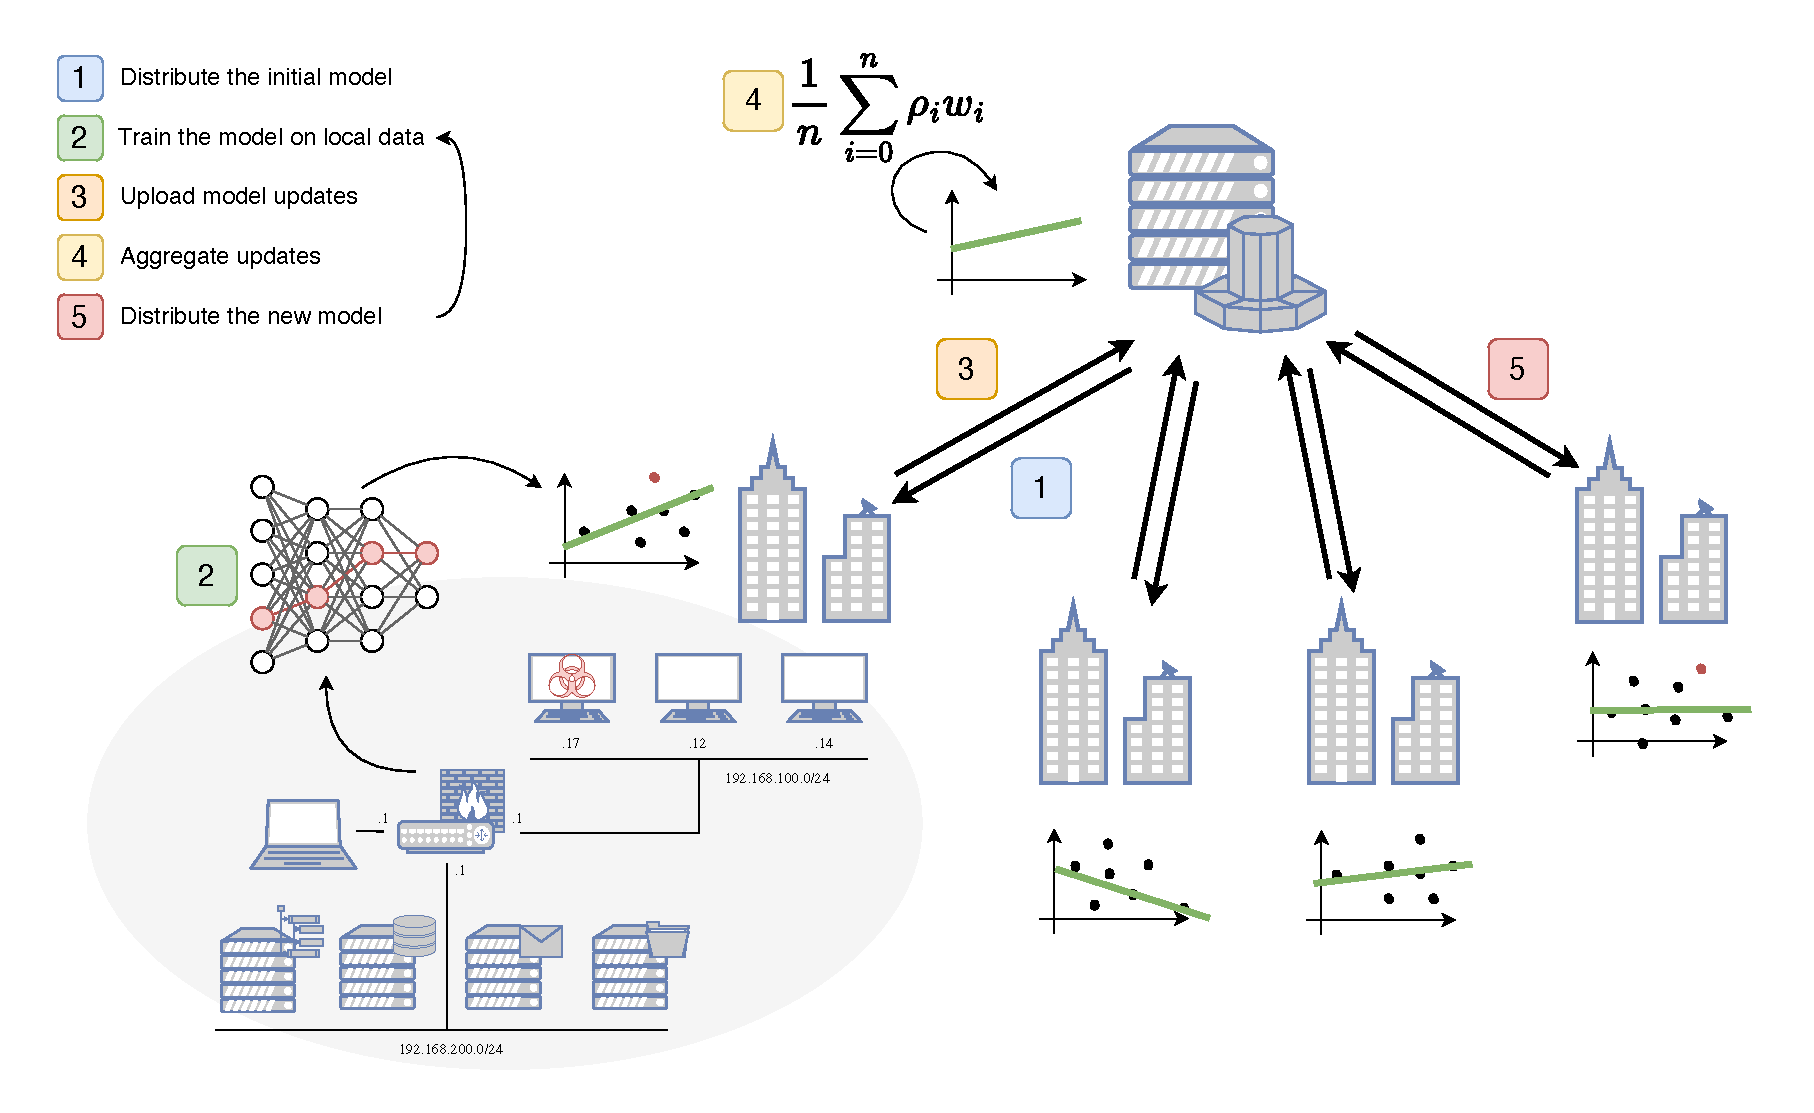
\includegraphics[width=\textwidth]{./figures/fids.drawio.pdf}
  \caption{Illustration of \gls{fl} in a \gls{cids} use case.}
  \label{fig:intro.usecase}
\end{figure}

\section{Research Objectives\label{sec:intro.questions}}

Overall, this work aims to answer the following: \emph{Can \gls{fl} serve as a trustable knowledge-sharing framework for collaboratively improving intrusion detection mechanisms \glspl{ids}?}
Based on the context and motivation laid out in the previous section, we formulize the general objectives of this dissertation as a set of research questions.
The questions stated hereafter are intended to be completed and extended in the following chapters, some of which introduce their own research questions.

Specifically, we globally focus on the following research questions:

\begin{questions}
  % 1. understand if FL can be used as a collaborative framework for IDS
  % - in which conditions
  % - to what extent
  % - what information can be shared
  \item What makes applying \gls{fl} to \glspl{ids} specific? \label{rq:intro.fids}
  % 2. Understand the impact of heterogeneity on FIDS
  \item Can \gls{fl} be used to federate \glspl{ids} across heterogeneous data sources? \label{rq:intro.heterogeneity}
  % 3. Understand and mitigate the effects of malicious contributions
  \item How does \gls{fl} handle malicious contributions in a federated \gls{ids}? \label{rq:intro.malicious}
  % 4. Assessing the trustworthiness of contributions
  \item How can one assess and ensure the trustworthiness of the other participants' contributions? \label{rq:intro.trust}
\end{questions}


\section{Contributions\label{sec:intro.contributions}}

We summarize the contributions of this dissertation as follows:

\begin{enumerate}
  \item The first \gls{slr} in literature that study the application of \gls{fl} to \gls{ids}. We propose a reference architecture and a taxonomy for structuring the domain, supported by quantitative and qualitative analyses of the existing literature.
  \item An illustrative study highlighting the challenges of heterogeneity and malicious contributions in \gls{fids}.
  \item An extensible evaluation framework for \glspl{fids} called Eiffel, leveraging popular open source libraries like Flower~\cite{beutel_Flowerfriendlyfederated_2020} and Hydra~\cite{Hydra}, and a set of malicious clients simulators. 
  \item A systematic analysis of the impact of label-flipping attacks on an \gls{fl}-based collaborative \gls{ids}, leveraging the aforementioned evaluation framework.
  \item A pioneer \gls{fl} architecture for collaborative \gls{ids} that handles malicious contributions in heterogeneous environments, leveraging a cross-evaluation mechanism and a reputation system.
  \item A methodology allowing to generate network topologies with heterogeneity constraints, and laying down the foundations toward a more realistic evaluation of \gls{fids} and distributed networking telemetry experiments in general.
\end{enumerate}


\section{Outline\label{sec:intro.outline}}

Apart from the introduction and conclusion chapters, the manuscript is organized in two parts: we define \glspl{fids} and identify their limitations in \Cref{part:fids}, before quantifying their limitations and providing solutions to address them in \Cref{part:contribs}.

\paragraph{\Cref{part:fids}:}

The first part delves into the application of \gls{fl} to \gls{ids}.
After layout out the necessary background in \Cref{chap:background}, we present the state of the art in \gls{fids} in \Cref{chap:sota}.
This chapter notably presents the results of our \gls{slr} on the topic, and focus on the related challenges and research opportunities.
\Cref{chap:application} then closes this first part by highlighting the main challenges in \gls{fids} using toy examples.

\paragraph{\Cref{part:contribs}:}

The second part presents our contributions to addressing the limitations of \gls{fids}.
\Cref{chap:assessment} introduces our evaluation framework, and systematically analyses the impact of label-flipping attacks on \gls{fids}, raising questions on the detection of malicious contributions in \gls{niid} settings.
To tackle these issue, \Cref{chap:radar} presents a pioneer \gls{fl} architecture for \gls{fids} that ensures the quality of incoming contributions in heterogeneous environments, with applications to the detections of malicious behaviors.
Finally, \Cref{chap:topologies} introduces a practical method to generate network topologies based on the composition of sub-topologies, and lays down the foundations for further studies on distributed intrusion detection.


\section{Publications\label{sec:intro.publications}}

\makeatletter
\newcommand\Setmaxbibnames[1]{\renewcommand\blx@maxbibnames{#1}}
\makeatletter

\begin{refsection}[biblio/lavaur.bib]
  \begin{refcontext}[sorting=ymdnt]
    \Setmaxbibnames{99}
    \nocite{*}
    \subsection*{Journal articles}
    \printbibliography[heading=none,type=article]
    \subsection*{International conference papers}
    \printbibliography[heading=none,type=inproceedings,keyword=confs]
    \subsection*{National conference papers}
    \printbibliography[heading=none,type=inproceedings,keyword=national]
    \subsection*{Tutorials}
    \printbibliography[heading=none,keyword=tutorial]
  \end{refcontext}
\end{refsection}